\chapter{Υλοποίηση Συστήματος}
\label{chap5}

Μέχρι στιγμής, έχει γίνει αναφορά στις τεχνολογίες και τις τεχνικές σχεδίασης της εφαρμογής. Το κεφάλαιο αυτό επεκτείνεται στην υλοποίηση της εφαρμογής, αναλύοντας τις μεθόδους που χρησιμοποίηθηκαν για τον προγραμματισμό τόσο του \tl{frontend}, όσο και του \tl{backend}. Η ενότητα 5.1 αφορά το \tl{frontend} κομμάτι, δηλαδή με τον προγραμματισμό των διεπιφανειών χρήστη. Η ενότητα 5.2 καταπιάνεται με την υλοποίηση του \tl{backend}, το οποίο απαρτίζεται από τον εξυπηρετητή αιτημάτων που δημιουργούνται από τις διεπιφάνειες χρήστη και τη βάση δεδομένων στην οποία αποθηκεύονται όλες οι πληροφορίες της εφαρμογής. Στην ενότητα 5.3 παρουσιάζονται τα τεχνολογικά εργαλεία τα οποία χρειάστηκαν στην υλοποίηση. Τέλος, στην ενότητα 5.4 γίνεται μια συνοπτική αναφορά στην πλοτφόρμα προγραμματισμού που επιλέχθηκε για την υλοποίηση της εφαρμογής. 


\section{Λεπτομέρειες Υλοποίησης Διεπιφανειών Χρήστη}
Ιδιαίτερο ενδιαφέρον παρουσιάζουν οι τεχνικές που χρησιμοποιήθηκαν στην υλοποίηση του συστήματος διεπιφανειών χρήστη. Η εφαρμογή αφορά κινητές συσκευές με λειτουργικό \tl{iOS}, επομένως δόθηκε μεγάλη βαρύτητα σε μεθόδους που υιοθετούν οι περισσότερες \tl{native} εφαρμογές της ίδιας κατηγορίας. Κατά τον προγραμματισμό, σχεδόν όλες οι διεπαφές που χρησιμοποιούνται αφορούν αποκλειστικά \tl{iOS} πλατφόρμες προκειμένου να προσφέρουν την καλύτερη δυνατή εμπειρία στο χρήστη.

Η εφαρμογή αναφέρεται σε κινητά τελευταίας γενιάς. Αυτό εισάγει κάποιους περιορισμούς στον προγραμματισμό, αλλά έχει ταυτοχρόνως και κάποια πλεονεκτήματα. Για παράδειγμα, οι διαστάσεις της οθόνης στις κινητές συσκευές είναι πολύ μικρότερες από αυτές ενός σταθερού υπολογιστή. Διαδραστικά στοιχεία όπως πλήκτρα, πεδία εισόδου, εικονίδια και άλλα γραφικά θα πρέπει να λαμβάνουν υπόψη τους τον παραπάνω περιορισμό. Συνεπώς, ο προγραμματισμός για \tl{mobile apps} είναι σαφώς πιο δύσκολος από τον προγραμματισμό για \tl{desktop apps}.

Το κυριότερο πλεονέκτημα του προγραμματισμού για να \tl{mobile apps} είναι το γεγονός ότι δεν χρειάζεται να δωθεί ιδιαίτερη βάση σε λεπτομέρειες, αφού οι οθόνες των κινητών δεν επιτρέπουν την σχολαστική ενασχόληση με κάθε στοιχείο ή την υπερβολική λεπτομέρεια των διαδραστικών στοιχείων, αφού αυτό θα καθιστούσε την εμπειρία χρήσης της εφαρμογής κουραστική για το χρήστη. Έτσι, ο προγραμματισμός επικεντρώνεται κυρίως γύρω από το κομμάτι με το οποίο θα αλληλιπιδρά ο χρήστης και τις τεχνικές λεπτομέρειες που συμπεριλαμβάνει. Για να εξασφαλιστεί μια ολοκληρωμένη, αλλά συγχρόνως απλή εμπειρία εντός της εφαρμογής, όλες οι διεπιφάνειες ακολουθούν αυτή την τακτική, όπου το διαδραστικό περιβάλλον αποτελείται αποκλειστικά από διεπαφές που είναι ζωτικές για την σωστή λειτουργία της κάθε οθόνης.


\subsection{Βασικά Προγραμματιστικά Χαρακτηριστικά Οθονών}
Βασική μέριμνα του προγραμματισμού των οθονών της εφαρμογής αποτέλεσε η χρήση οικουμενικών διεπαφών. Η δυνατότητα επαναληψημότητας ορισμένων προγραμματιστικών τεχνικών, συνέβαλλε στην απλοποίηση της διαδικασίας υλοποίησης και την ευκολία χειρισμού των διεπιφανειών. Τα κυριότερα χαρακτηριστικά των διεπαφών αυτών είναι η χρήση ενός κεντρικού πλοηγητή για την περιήγηση στις οθόνες της εφαρμογής, η επικεφαλίδες με τίτλο για την κάθε οθόνη, η ύπαρξη ενός κεντρικού μενού πλοήγησης σελίδων και τα βασικά πλήκτρα ενεργειών στην επικεφαλίδα κάθε οθόνης (βλ. Σχ. \ref{example}). Καθένα από τα παραπάνω προγραμματιστικά χαρακτηριστικά αναλύεται στη συνέχεια.

\begin{figure}[H]
    \centering
    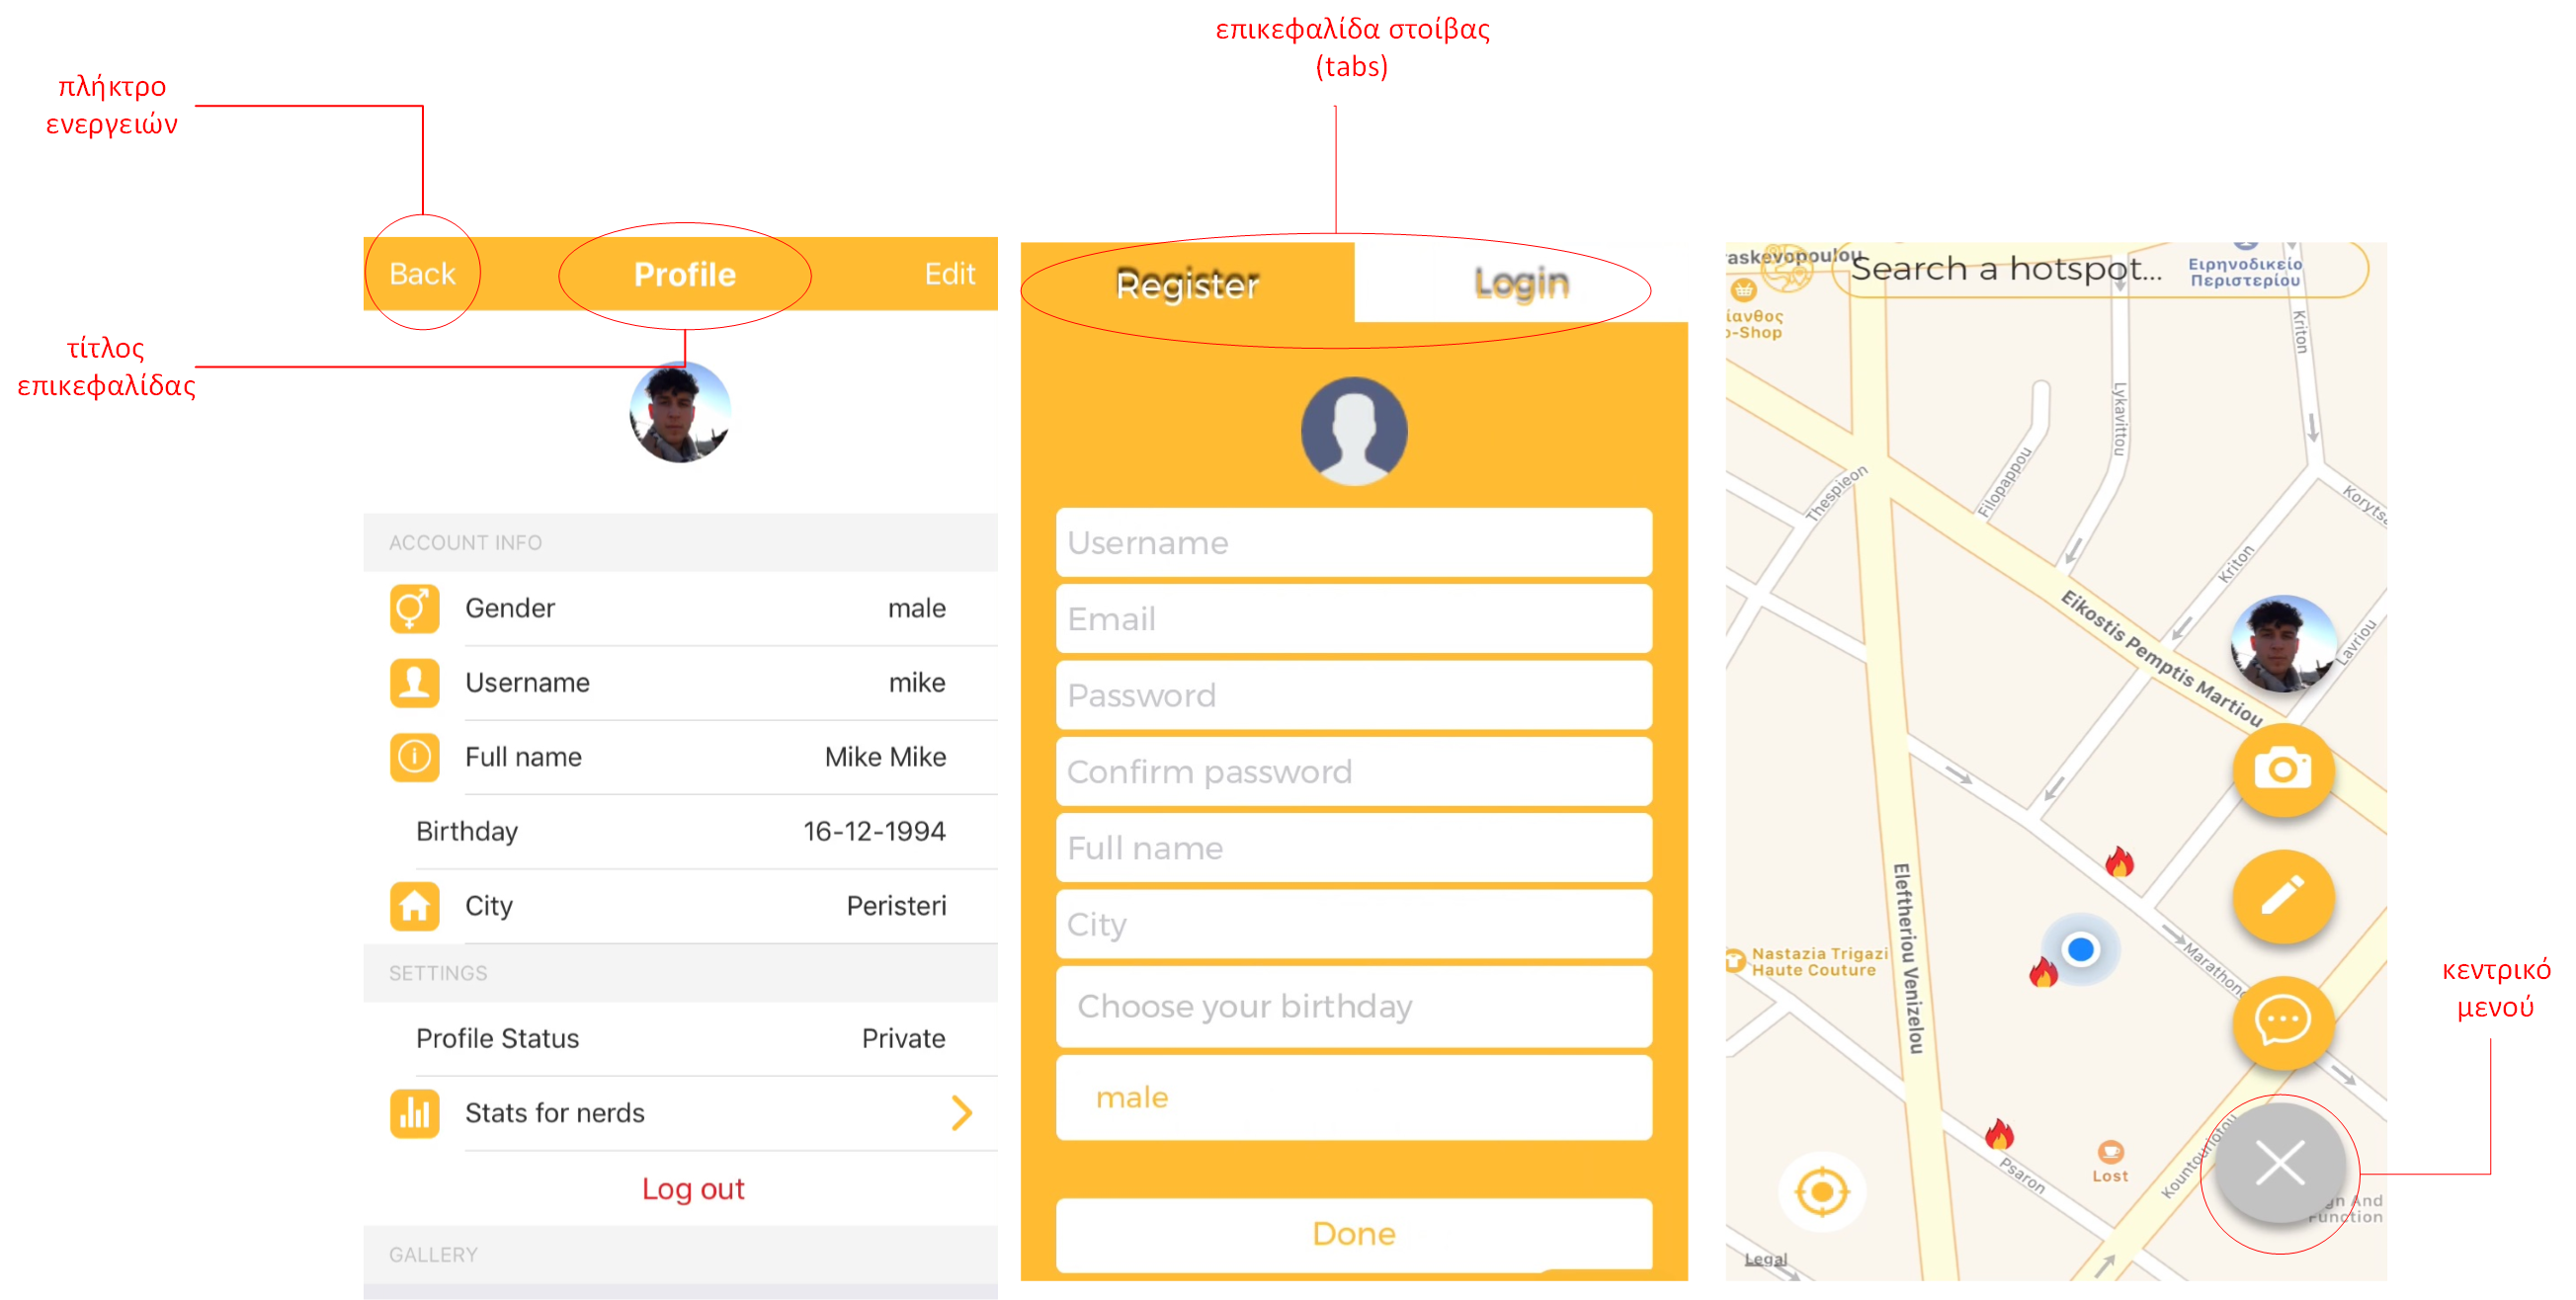
\includegraphics[scale=0.2]{figures/exaple.png}
    \caption{Παράδειγμα χαρακτηριστικών που επαναλαμβάνονται σε όλη την εφαρμογή.}
    \label{example}
\end{figure}

\subsubsection{Τεχνική Πλοήγησης στην Εφαρμογή}
Ένα από τα βασικότερα σημεία της υλοποίησης αποτελεί η πλοήγηση εντός της εφαρμογής. Η τεχνική που ακολουθήθηκε βασίζεται στην ύπαρξη ενός ενιαίου \tl{router}, ο οποίος είναι υπευθυνος για την πλόγηση κάθε φορά στην επιλεγμένμη σελίδα, αλλά και την αποθήκευση της σελίδας σε μια στοίβα. Με αυτό τον τρόπο, είναι δυνατή η εκτεταμένη περιήγηση σε περισσότερες από μια σελίδες της εφαρμογής και η επιστροφή σε οποιαδήποτε από τις προηγούμενες σελίδες χάρις την δυνατότητα διευθυνσιοδότητησης καθεμιάς από τις σελίδες αυτές.
\newline
\indent
Πρακτικά, αυτό επιτυγχάνεται με την τεχνική των εμφωλευμένων σελίδων. Σύμφωνα με αυτή, οι σελίδες που πρόκειται να έχουν τη δυνατότητα επιστροφής σε κάποια προηγούμενη σελίδα θα εμφωλιάζονται ομαδικά υπό μια υποτιθέμενη ``\textit{σκηνή}'' (\tl{scene}). Κάθε σελίδα αποτελεί από μόνη της μια σκηνή και πολλές σκηνές μαζί δημιουργούν μια ``\textit{στοίβα}'' από σκηνές (\tl{stack}). Όσες σκηνές βρίσκονται εντός της στοίβας, μπορούν να διαδέχονται η μία την αμέσως επόμενη, έχοντας ταυτόχρονα την δυνατότητα επιστροφής στην προηγούμενη σελίδα-σκηνή. Επίσης, υιοθετούν μία σειρά από ιδιότητες στις οποίες θα γίνει αναφορά στις ενότητες που ακολουθούν.
\newline
\indent
Όλες οι στοίβες που θα δημιουργηθούν τελικά, είναι εμφωλευμένες στον \tl{router}. Αν το τελευταίο δεν ισχύει, τότε οι παραπάνω ιδιότητες δεν εφαρμόζονται στις επιμέρους στοίβες.


\subsubsection{Επικεφαλίδα Οθόνης}
 Μία από τις βασικότερες ίσως ιδιότητες που μεταδίδεται στις σκηνές που απαρτίζουν μια στοίβα είναι η επικεφαλίδα. Κάθε οθόνη που ανήκει στην ομάδα εμφωλευμένων σκηνών έχει την δυνατότητα να φέρει ή όχι κάποια χαρακτηριστικά στην επικεφαλίδα. Αυτά είναι η επιπλέον επικεφαλίδα της στοίβας, αποκλειστικές σχεδιαστικές επεμβάσεις (όπως πχ. χρώμα, είδος και μέγεθος γραμματοσειράς, εικονίδια κλπ.),  ο τίτλος της παρούσας σελίδας, διαρρύθμιση πλήκτρων που θα έχει η επικεφαλίδα, αλλαγή θέσης των στοιχείων και πολλά άλλα. Η επικεφαλίδα αποτελεί ξεχωριστό \tl{component}, το οποίο ανήκει σε μια ομάδα επαναχρησιμοποιήσιμων \tl{components} (\tl{commons}) και χρησιμοποιείται σε κάθε σελίδα με διαφορετικές διαρρυθμίσεις.
 \newline
\indent
Οι παραπάνω ιδιότητες είναι ιδιαίτερα χρήσιμες στον προγραμματισμό κάθε οθόνης. Δίνουν πολλές επιλογές στον προγραμματιστή όσον αφορά στην διαμόρφωση της επικεφαλίδας της κάθε οθόνης και την ανεξαρτητοποίηση των οθονών μεταξύ τους από  σχεδιαστικής απόψεως. Από την άλλη, μπορούν να αυτοματοποιηθούν πολλές προγραμματιστικές ενέργειες με την χρήση τμημάτων κώδικα που μπορεί να επαναχρησιμοποιηθεί σε όλες σχεδόν τις οθόνες. Αυτό καθιστά τη διαδικασία προγραμματσιμού αισθητά πιο εύκολη και βέλτιση.

\subsubsection{Κεντρικό Μενού Οθονών}
Στη δεξιότερη εικόνα του σχ. \ref{example} φαίνεται το κεντρικό μενού για την πλοήγηση μεταξύ των οθονών της εφαρμογής. Η τεχνική χρήσης ενός κεντρικού πλήκτρου για όλες τις βασικές οθόνες της εφαρμογής επιλύει πολλά προβλήματα και καθιστά το κομμάτι του προγραμματισμού αρκετά πιο απλό. Το \tl{FAB} εξυπηρετεί επίσης από άποψη χώρου, αφού δεν καταλαμβάνει μεγάλο τμήμα της  κεντρικής οθόνης, πράγμα που το κάνει την καταλληλότερη προγραμματιστική τεχνική. Μια άλλη προσέγγιση θα ήταν η ύπαρξη μιας μπάρας εικονιδίων με τις κύριες οθόνες στο κάτω μέρος της οθόνης, αλλά αυτό θα μείωνε αρκετά τις διαστάσεις της διεπαφής χάρτη, που είναι άλλωστε και το κύριο χαρακτηριστικό της οθόνης.
\newline
\indent
Το \tl{FAB} αποτελεί ξεχωριστό \tl{component} της κεντρικής οθόνης και συνίσταται από το κύριο πλήκτρο επέκτασης του μενού και τρία επιμέρους εικονίδια. Κάθε εικονίδιο αντιστοιχεί και σε μία από τις βασικές οθόνες της εφαρμογής και για τον λόγο αυτό του έχει αποδωθεί κατάλληλο εικονίδιο.


\subsubsection{Βασικά Πλήκτρα Ενεργειών}
Όπως έχει ήδη αναφερθεί, κάθε οθόνη διαθέτει μια εξατομικευμένη επικεφαλίδα. Η επικεφαλίδα, εκτός των άλλων φέρει τον τίτλο της σελίδας στον οποίο βρίσκεται ο χρήστης και κάποια βασικά πλήκτρα ενεργειών. Τα πλήκτρα αυτά αποσκοπούν στην δυνατότητα πλοήγησης προς τα εμπρός ή προς τα πίσω σε μια στοίβα σελίδων. Για παράδειγμα, όταν ο χρήστης επισκέπτεται την οθόνη του προσωπικού του \tl{profile} (\tl{ProfileScreen}), μπορεί είτε να επιστρέψει στην προηγούμενη σελίδα πατώντας το πλήκτρο επιστροφής με την επιγραφή ``\textit{\tl{back}}'', είτε να πλοηγηθεί στην σελίδα επεξεργασίας των προσωπικών του στοιχείων (\tl{EditProfileScreen}) πατώντας το πλήκτρο επιστροφής με την επιγραφή ``\textit{\tl{edit}}''.
\newline
\indent
ο προγραμματισμός της λειτουργικότητας του κάθε πλήκτρου ενεργειών εξαρτάται από το είδος της σελίδας. Το πλήκτρο στα αριστερά μιας σελίδας έχει πάντοτε το ρόλο επιστροφής στην προηγούμενη σελίδα. Ανάλογα με τις ενέργειες που θα παρέχονται στον χρήστη, το πλήκτρο ενεργειών στα δεξιά της επικεφαλίδας θα εκτελεί είτε την λειτουργία επεξεργασίας δεδομένων, είτε τη λειτουργία υποβολής φόρμας. Στο παραπάνω παράδειγμα, η οθόνη στην οποία αναφέρονται τα πλήκτρα ενεργειών είναι αυτή του \tl{profile} του χρήστη, επομένως το πλήκτρο στα αριστερά παίζει το ρόλο της επιστροφής στην προηγούμενη σελίδα, ενώ το πλήκτρο στα δεξιά μεταφέρει το χρήστη στην οθόνη επεξεργασίας. Εκεί έπειτα, τα πλήκτρα αναφέρονται σε μια οθόνη που περιέχει φόρμα, συνεπώς το πλήκτρο στα δεξιά έχει τώρα τον ρόλο υποβολής της φόρμας. 

\subsection{Λειτουργικότητα Οθονών Εφαρμογής}
Στην ενότητα αυτή θα αναλυθούν οι μεθοδολογίες που ακολουθήθηκαν στην υλοποίηση των λειτουργικοτήτων της εφαρμογής. Όπως αναφέρθηκε ήδη στο Κεφ. 3, η εφαρμογή θα δίνει στο χρήστη τη δυνατότητα εγγραφής και σύνδεσης στην εφαρμογή, ως μέσο ταυτοποίησης. Ακόμη, ο χρήστης θα μπορεί να πλοηγείται σε ένα χάρτη στα διάφορα σημεία ενδιαφέροντος. Εκεί, θα μπορεί να επιλέξει από μια πληθώρα ενεργειών για να αλληλεπιδράσει με τα στοιχεία του χάρτη. Η εφαρμογή θα δίνει στο χρήστη τη δυνατότητα να εξατομικεύσει τον προσωπικό του λογαριασμό, μέσα από την ταξιθέτηση των προσωπικών του δημοσιεύσεων αλλά και από την επεξεργασία του προσωπικού του \tl{profile}. Τέλος, ο χρήστης θα μπορεί να αποσυνδεθεί απο την εφαρμογή όποτε το επιθυμεί.
 


\subsubsection{\tl{RegisterScreen \& LoginScreen}}
Η οθόνη αποτελείται από δύο επιμέρους \tl{tabs}, ένα για εγγραφή και ένα για σύνδεση των χρηστών. Ο χρήστης μπορεί να επιλέγει κάθε φορά το \tl{tab} που αρμόζει στην στην κάθε περίπτωση. Εάν ο χρήστης επιθυμεί να πραγματοποιήσει εγγραφή στην εφαρμογή, μπορεί να επιλέξει το \tl{tab} με τίτλο ``\textit{\tl{Register}}'', κάνοντας \tl{swipe} προς τα δεξιά. Από την άλλη, εάν ο χρήστης θέλει να πραγματοποιήσει σύνδεση στον λογαριασμό του, μπορεί να επιλέξει το \tl{tab} με τίτλο ``\textit{\tl{Login}}'', κάνοντας \tl{swipe} προς τα αριστερά.
\newline
\indent
Κάθε οθόνη περιέχει μια φόρμα με πεδία τα οποία καλείται να συμπληρώσει ο χρήστης. Στην οθόνη εγγραφής, η φόρμα περιέχει πεδία για το πλήρες όνομα, το όνομα χρήστη, την ηλεκτρονική διεύθυνση, τον κωδικό πρόσβασης, την πόλη, το γένος και την ημερομηνία γέννησης του χρήστη. Επίσης, ο χρήστης μπορεί να επιλέξει μία από τις φωτογραφίες στη συλλογή του ή να βγάλει μια νέα φωτογραφία και να την θέσει ως εικόνα προφίλ στο λογαριασμό του. Η οθόνη σύνδεσης είναι πιο σύντομη και αποτελείται από δύο πεδία, τα οποία ο χρήστης συμπληρώνει με τα διαπιστευτήριά του. Ο συνδυασμός διαπιστευτηρίων χρήστη αποτελείται από την ηλεκτρονική διεύθυνση και των κωδικό πρόσβασης του χρήστη. Σε καθεμία εκ των ανωτέρω περιπτώσεων, ο χρήστης μεταφέρεται στο χάρτη της κεντρικής οθόνης της εφαρμογής μετά από επιτυχή υποβολή της φόρμας.
\newline
\indent
Κάθε φόρμα έχει υλοποιηθεί ώστε να προσφέρει την καλύτερη δυνατή εμπειρία χρήστη. Το είδος της εισόδου που απαιτείται στην συμπλήρωση κάθε φόρμας διαφέρει από πεδίο σε πεδίο. Για παράδειγμα, το πεδίο κωδικού πρόσβασης απαιτεί είσοδο αποτελούμενη από αλφαριθμητικούς χαρακτήρες, ενώ στο πεδίο της ηλεκτρονικής διεύθυνσης χρησιμοποιούνται συγκεκριμένοι ειδικοί χαρακτήρες και σύμβολα. Για το λόγο αυτό, έχει προσιοριστεί το είδος κάθε πεδίου, με αποτέλεσμα την εμφάνιση του κατάλληλου είδους πληκτρολογίου κάθε φορά. Επίσης, το πλήκτρα υποβολής κάθε φόρμας αντικαθίστανται από \tl{spinners} που δείχνουν στο χρήστη ότι η εφαρμογή φορτώνει.
\newline
\indent
Σε περίπτωση ανεπιτυχούς υποβολής κάποιας από τις παραπάνω φόρμες, η εφαρμογή ενημερώνει το χρήστη σχετικά με τη φύση του σφάλματος. Σφάλματα μπορούν να προκύψουν από την λανθασμένη συμπλήρωση ενός ή περισσότερων πεδίων εισόδου. Σε κάθε περίπτωση, ένα κατάλληλο μήνυμα λάθους εμφανίζεται κάτω από το αντίστοιχο πεδίο, το οποίο αναφέρει συνοπτικά τις μετατροπές που πρέπει να γίνουν ώστε να είναι αποδεκτή η είσοδος του χρήστη. 

\subsubsection{\tl{HomeScreen}}

Σε αυτό το σημείο της εφαρμογής εμφανίζονται και οι κατάλληλες ειδοποιήσεις στο χρήστη. Η εφαρμογή χρείαζεται την τοποθεσία του χρήστη για να την προσδιορίσει στο χάρτη και στη συνέχεια να φορτώσει τα \tl{hotspots}. Δίνοντας την συγκατάνευσή του, ο χρήστης επιτρέπει στην εφαρμογή να πραγματοποιήσει τις αναγκαίες ρυθμίσεις για την ορθή λειτουργία της. Επίσης, ο χρήστης θα πρέπει να πραγματοποιήσει σύνδεση σε κάποιο δίκτυο προκειμένου να μπορέσει να χρησιμοποιήσει την εφαρμογή.
\newline
\indent
Μετά την είσοδό του στην εφαρμογή, ο χρήστης ανακατευθύνεται στον χάρτη. Ο χάρτης φορτώνει με τα \tl{hotspots} που βρίσκονται εντός εμβέλειας της τοποθεσίας του χρήστη. Η εμβέλεια είναι προγραμματισμένη να έχει μία ακτίνα ίση με \tl{5km}. Τα \tl{hotspots} που φαίνονται στο χάρτη και έχουν δημιουργηθεί από άλλους χρήστες συμβολίζονται με \tl{markers} που έχουν τη μορφή φωτιάς συγκεκριμένου μεγέθους. Το μέγεθος κάθε \tl{marker} ποικίλλει και εξαρτάται από τον αριθμό προβολών του \tl{hotspot}. Οσο πιο πολλοί χρήστες έχουν δει ένα συγκεκριμένο \tl{hotspot}, τόσο μεγαλύτερο είναι το μέγεθος της φωτιάς. Έτσι, δημιουργείται μια αναλογία μεταξύ των \tl{hotspots} και του ενδιαφέροντος των χρηστών.
\newline
\indent
Ο χρήστης μπορεί να επιλέξει να προβάλλει ένα \tl{hotspot} από το χάρτη. Πατώντας επάνω στο \tl{marker} του \tl{hotspot}, θα εμφανιστεί ένα πλαίσιο (\tl{callout}), το οποίο περιέχει τις κυριότερες πληροφορίες που σχετίζονται με το συγκεκριμένο \tl{hotspot}. Στο πλαίσιο φαίνεται συνοπτικά ένα τμήμα της περιγραφής του \tl{hotspot}, το όνομα και η εικόνα προφίλ του χρήστη που έχει αναρτήσει το \tl{hotspot}, ο χρόνος που έχει περάσει από την ώρα ανάρτησης, και ο αριθμός προβολών και σχολίων του \tl{hotspot}. 
\newline
\indent
Στην οθόνη χάρτη υπάρχουν τέσσερεις επιπλέον διεπαφές. Η μπάρα αναζήτησης, το κρυφό συρταρωτό μενού, το πλήκτρο επαναφοράς τοποθεσίας χρήστη και το κεντρικό πλήκτρο πλοήγησης. Το πλήκτρο επαναφοράς τοποθεσίας χρήστη βρίσκεται στο κάτω αριστερά μέρος της οθόνης. Όπως φανερώνει και το όνομά του, βοηθάει το χρήστη να επαναφέρει τη θέση του χάρτη στην τοποθεσία την οποία βρίσκεται εκείνη τη στιγμή. Το κεντρικό πλήκτρο πλοήγησης βρίσκεται στο κάτω δεξιά μέρος της οθόνης και πατώντας το ο χρήστης μπορεί να επιλέξει σε ποια οθόνη θέλει να μεταφερθεί. Για τις άλλες δύο διεπαφές θα γίνει μια πιο εκτεταμένη αναφορά στη συνέχεια. 

\paragraph{Μπάρα Αναζήτησης και \tl{Foursquare Suggest Completion}}
\paragraph{}
Εάν ο χρήστης επιθυμεί να πραγματοποιήσει μια συγκεκριμένη αναζήτηση ενός σημείου ενδιαφέροντος, μπορεί να το κάνει μέσω της μπάρας αναζήτησης στο πάνω μέρος της οθόνης. Ο χρήστης πληκτρολογεί λέξεις-κλειδιά που σχετίζονται με την τοποθεσία προς αναζήτηση, όπως το όνομα, την περιοχή κλπ. Η διεπαφή είναι εφοδιασμένη με την ιδιότητα αυτοσυμπλήρωσης του \tl{Foursquare API}. Συνεπώς, τα αποτελέσματα εμφανίζονται καθώς ο χρήστης πληκτρολογεί, σε μια λίστα ακριβώς κάτω από την μπάρα. 
\newline
\indent
 Το \tl{Foursquare API}, όπως αναφέρθηκε στην ενότητα 2.2.2, είναι μια διεπαφή ανοικτού κώδικα η οποία χρησιμεύει στην εύρεση πληροφοριών για διάφορα μέρη. Στην εφαρμογή, ένα από τα σημεία στα οποία ενσωματώνεται η διεπαφή αυτή είναι η μπάρα αναζήτησης στο επάνω μέρος του χάρτη, για την αυτοσυμπλήρωση των εμφανιζόμενων αποτελεσμάτων. Όταν πραγματοποιείται αναζήτηση, η είσοδος του χρήστη προστίθεται στο προς αναζήτηση \tl{URL} και η εφαρμογή δημιουργεί ένα αίτημα \tl{GET} προς την διεπαφή \tl{Foursquare API Suggest Completion}
 
\hfill
\begin{mdframed}[backgroundcolor=lightgrey] 
 \tl{\ttfamily{GET https://api.foursquare.com/v2/venues/suggestcompletion}}   
\end{mdframed}
\hfil

\noindent  επισυνάπτοντας τις λέξεις-κλειδιά και κάποια ακόμη δεδομένα ως \tl{endpoint} στο παραπάνω \tl{URL}, για την λήψη των απαιτούμενων πληροφοριών του σημείου ενδιαφέροντος. Το αποτέλεσμα είναι η εμφάνιση προτεινόμενων σημείων ανδιαφέροντος καθώς ο χρήστης πληκτρολογεί την επιθυμητή είσοδο.  

Το αίτημα που τελικά αποστέλλεται στο \tl{Foursquare API} αποτελείται από ένα νέο \tl{URL}, το οποίο περιλαμβάνει τα απαραίτητα στοιχεία για την εύρεση των σχετικών αποτελεσμάτων. Το νέο \tl{URL} που δημιουργείται, εμπεριέχει το παραπάνω \tl{URL}, μαζί με ένα \tl{query} που περιλαμβάνει τις εξής παραμέτρους αναζήτησης:

\begin{itemize}
    \item \textbf{\textit{\tl{ll}}} \textbf{--} η παράμετρος αυτή προσδιορίζει την τοποθεσία στην οποία γίνεται η αναζήτηση
    \item \textbf{\textit{\tl{query}}} \textbf{--} οι λέξεις-κλειδιά που πληκτρολογεί ο χρήστης
    \item \textbf{\textit{\tl{limit}}} \textbf{--} η παράμετρος αυτή προσδιορίζει την πλήθος των εμφανιζόμενων αποτελεσμάτων
    \item \textbf{\textit{\tl{radius}}} \textbf{--} η παράμετρος αυτή προσδιορίζει την ακτίνα αναζήτησης σε \tl{m}
    \item \textbf{\textit{\tl{v}}} \textbf{--} η παράμετρος αυτή προσδιορίζει την \tl{version} της διεπαφής
\end{itemize}


Στον πίνακα που ακολουθεί, γίνεται ανάλυση ενός παραδείγματος για την καλύτερη κατανόηση του τρόπου λειτουργίας της διεπαφής αυτοσυμπλήρωσης.

\begin{table}[h]
\centering
\begin{tabular}{ |m{2cm}|m{2cm}|m{8cm}|  }
\hline
\multicolumn{3}{|c|}{\selectlanguage{english}Search Example: Acropolis Museum\selectlanguage{greek}} \\
\hline 
\textit{\tl{\textbf{Name}}} & \textit{\tl{\textbf{Example}}} & \textit{\tl{\textbf{Description}}}  \\
\hline 
\tl{\textit{ll}}
 & \tl{37.8,23.2} & \tl{\textbf{required} latitude and longitude of the user’s location.}\\
\hline
\tl{\textit{query}}
 & \tl{acropolis museum} & \tl{\textbf{required} search term to be applied against titles. Must be at least 3 characters long.}\\
 \hline
 \tl{\textit{limit}}
 & \tl{20} & \tl{number of results to return, up to 50.}\\
 \hline
 \tl{\textit{radius}}
 & \tl{800} & \tl{limit results to venues within this many meters of the specified location. Defaults to a city-wide area. The maximum supported radius is currently 80,000 meters.}\\
\hline
 \tl{\textit{v}}
 & \tl{20190501} & \tl{the current API version.}\\
\hline
 \tl{\textit{client\_id}}
 &  & \tl{a \textbf{unique} string that is given to the client for access privileges.}\\
\hline
 \tl{\textit{client\_secret}}
 &  & \tl{a \textbf{unique} string that is given to the client for access privileges.}\\
\hline
\end{tabular}
\selectlanguage{greek}
\caption{Παράδειγμα αυτοσυμπλήρωσης για τις λέξεις-κλειδιά \tl{acropolis museum} και δομή του \tl{URL} αναζήτησης.}
\label{tab:parameters}
\end{table}


\paragraph{Συρταρωτό Μενού και \tl{Foursquare Explore}}
\paragraph{}
Στις δυνατότητες του χρήστη συμπεριλαμβάνεται και η φιλτραρισμένη αναζήτηση σημείων ενδιαφέροντος. Εάν ο χρήστης επιθυμεί να προβάλλει στο χάρτη σημεία που ανήκουν σε κάποια συγκεκριμένη κατηγορία, μπορεί να το κάνει, ανοίγοντας το κρυφό συρταρωτό μενού πατώντας το εικονίδιο της υδρόγειου σφαίρας στο επάνω αριστερά μέρος του χάρτη, ή σύροντας την οθόνη προς τα δεξιά. Στη συνέχεια, μπορεί να επιλέξει μία από τις κατηγορίες της λίστας και τα αποτελέσματα θα εμφανιστούν στο χάρτη. 
\newpage
Η παραπάνω υπηρεσία υλοποιείται με τη χρήση της διεπαφής \tl{Foursquare Explore}, με βάση την οποία η εφαρμογή δημιουργεί αιτήματα αναζήτησης σημείων ενδιαφέροντος που ανήκουν σε κάποια από τις διαθέσιμες κατηγορίες. Τα αιτήματα που δημιουργούνται έχουν την ακόλουθη μορφή

\begin{mdframed}[backgroundcolor=lightgrey] 
 \tl{\ttfamily{GET https://api.foursquare.com/v2/venues/search}}   
\end{mdframed}

\noindent και το \tl{URL} εμπεριέχει κάποιες επιπρόσθετες παραμέτρους που συνιστούν το \tl{query} προς αποστολή στην διεπαφή. Στη συνέχεια θα αναλυθεί ένα παράδειγμα των αποτελεσμάτων που επιστρέφονται στην εφαρμογή από τη διεπαφή, όταν ο χρήστης επιλέγει την κατηγορία με ετικέτα ``\textit{\tl{arts}}''.
\newline
\indent
Το νέο \tl{URL} που θα δημιουργηθεί θα ξεκινάει με το παραπάνω \tl{URL} και θα περιέχει κάποιες ακόμη πληροφορίες που θα συνιστούν το τελικό \tl{endpoint}. Οι πληροφορίες αυτές είναι παρόμοιες με αυτές που χρησιμοποιήθηκαν για το σχηματισμό του \tl{endpoint} που θα αποσταλλεί στη διεπαφή \tl{Foursquare Suggest Completion}, με μία μόνο επιπλέον παράμετρο: την κατηγορία (\tl{section}) στην οποία ανήκει το σημείο ενδιαφέροντος, για τον περιορισμό της αναζήτησης. Στο παράδειγμα όπου ο χρήστης επιλέγει σαν φίλτρο της αναζήτησης την κατηγορία ``\textit{\tl{arts}}'', τότε η παράμετρος \tl{section} αντιστοιχίζεται με την κατηγορία \tl{arts}.
\newline
\indent
Τα αποτελέσματα που επιστρέφει η διεπαφή \tl{Foursquare Explore} θα περιέχουν μια σειρά από πληροφορίες, τις οποίες η εφαρμογή θα διαχειρίζεται κατάλληλα για την εμφάνισή τους στο χάρτη. Τα στοιχεία που επιστρέφονται από τη διεπαφή φαίνονται στον κάτωθι πίνακα:

\begin{table}[h]
\centering
\begin{tabular}{ |m{2cm}|m{10cm}|  }
\hline
\multicolumn{2}{|c|}{\tl{https://api.foursquare.com/v2/venues?ll=37.8,23.7\&section=arts\&radius=800}} \\
\hline 
\textit{\tl{\textbf{Field}}} & \textit{\tl{\textbf{Description}}}  \\
\hline 
\tl{\textit{id}}
 & \tl{a \textbf{unique} string identifier for this venue.}\\
\hline
\tl{\textit{name}}
 & \tl{the best known name for this venue.}\\
 \hline
 \tl{\textit{location}}
 & \tl{an object containing none, some, or all of address (street address), crossStreet, city, state, postalCode, country, lat, lng, and distance. All fields are strings, except for lat, lng, and distance. Distance is measured in meters. Some venues have their locations intentionally hidden for privacy reasons (such as private residences). If this is the case, the parameter isFuzzed will be set to true, and the lat/lng parameters will have reduced precision.}\\
 \hline
 \tl{\textit{categories}}
  & \tl{an array, possibly empty, of categories that have been applied to this venue. One of the categories will have a primary field indicating that it is the primary category for the venue. For the complete category tree, see categories.}\\
\hline
\end{tabular}
\selectlanguage{greek}
\caption{πληροφορίες που επιστρέφονται από τη διεπαφή \tl{Foursquare Explore}.}
\label{tab:parameters}
\end{table}

Εκτός από την αναζήτηση σημείων ενδιαφέροντος, ο χρήστης μπορεί να προβάλλει κάποια από τα \tl{hotspots} που εμφανίζονται στο χάρτη. Πατώντας επάνω σε κάποιο \tl{marker}, ο χρήστης μπορεί να δει τις πληροφορίες που αφορούν το συγκεκριμένο \tl{hotspot}, όπως να διαβάσει την περιγραφή, να δει το χρήστη που δημιούργησε το \tl{hotspot}, να δει τον αριθμό σχολίων ή προβολών κλπ. 


\subsubsection{\tl{CreateHotspotScreen}}
Για τη δημιουργία ενός προσωπικού \tl{hotspot}, ο χρήστης μεταφέρεται στην οθόνη \tl{CreateHotspotScreen}. Εκεί, μπορεί να δώσει στο νέο του \tl{hotspot} μια περιγραφή, να θέσει χρόνικό όριο ισχύος και να επισυνάψει μια φωτογραφία από τη συλλογή της συσκευής του ή να βγάλει καινούρια με την κάμερα. Μόλις ολοκληρώσει τη συμπλήρωση της φόρμας δημιουργίας με τα παραπάνω στοιχεία, ο χρήστης πατάει το πλήκτρο με επιγραφή ``\textit{\tl{Done}}'' που βρίσκεται στο δεξιά μέρος της επικεφαλίδας της οθόνης.
\newline
\indent
Σε περίπτωση σφάλματος, η διεπαφή μηνυμάτων λάθους αναλαμβάνει την εμφάνιση κατάλληλου μηνύματος προς το χρήστη. Το μήνυμα θα έχει τη μορφή ειδοποιητικού πλαισίου διαλόγου, όπου και θα περιγράφεται το αίτιο που προξενεί το σφάλμα στη φόρμα δημιουργίας \tl{hotspot}. Στη συνέχεια, ο χρήστης αποδέχεται την ειδοποίηση πατώντας ``\textit{\tl{OK}}'' και προχωράει στη διόρθωση των σφαλμάτων. Το πεδίο περιγραφής του \tl{hotspot} δεν πρέπει να είναι κενό, ενώ η τιμή χρονικού ορίου αρχικοποιείται στα 30 λεπτά. Η προσθήκη φωτογραφίας είναι προαιρετική. Ο χρήστης μπορεί να ακυρώσει τη δημιουργία του νέου \tl{hotspot} ανά πάσα στιγμη πατώντας το πλήκτρο με επιγραφή ``\textit{\tl{Cancel}}'' που βρίσκεται στα αριστερά της επικεφαλίδας της οθόνης.
\newline
\indent
Μόλις η φόρμα δημιουργίας νέου \tl{hotspot} διορθωθεί και δεν περιέχει άλλα λάθη, η υποβολή ολοκληρώνεται επιτυχώς. Ο χρήστης ενημερώνεται για τις ενέργειες που θα ακολουθήσουν μετά την υποβολή της φόρμας και καλείται να αποδεχθεί ή όχι την δημιουργία του νέου \tl{hotspot}. Εάν ο χρήστης αποδεχθεί τη δημιουργία του νέου \tl{hotspot}, τότε ανακατευθύνεται στο χάρτη και το καινούριο \tl{hotspot} αποθηκεύεται στη βάση και εμφανίζεται στο χάρτη στην τοποθεσία του χρήστη. Διαφορετικά, το \tl{hotspot} δεν αποθηκεύεται και ο χρήστης μεταφέρεται ξανά στο χάρτη.


\subsubsection{\tl{HotspotListScreen}}
Η εξατομίκευση της εφαρμογής ανάλογα με το χρήστη επιτυγχάνεται με την λίστα προσωπικών \tl{hotspots} στην \tl{HotspotListScreen}. Εκεί, μπορεί να μεταφερθεί ο χρήστης όταν επιθυμεί να προβάλλει όλα τα προσωπικά \tl{hotspots} που έχει δημιουργήσει στο παρελθόν. Η λίστα είναι ταξινομημένη με τα πιο πρόσφατα  \tl{hotspots} να εμφανίζονται πρώτα και τα παλαιότερα να βρίσκονται στο τέλος. 
\newline
\indent
Η οθόνη προσωπικών  \tl{hotspots} εξυπηρετεί επίσης στην διευκόλυνση της διαδικασίας διαχείρισης των  \tl{hotspots} του χρήστη. Εάν ο χρήστης επιθυμεί να επεξεργαστεί την περιγραφή κάποιου \tl{hotspot} για παράδειγμα, μπορεί να το κάνει από εδώ. Η διαδικασία είναι απλή και σύντομη, αφού ο χρήστης απλώς σύρει το συγκεκριμένο \tl{hotspot} προς τα δεξιά και πατάει το πλήκτρο με την επιγραφή ``\tl{\textit{edit}}''. Στην σελίδα επεξεργασίας, ο χρήστης μπορεί να μεταβάλλει όλες τις πληροφορίες που σχετίζονται με το \tl{hotspot}. Μπορεί επίσης να αλλάξει την εικόνα του \tl{hotspot}, ή να προσθέσει μια εικόνα σε περίπτωση που δεν υπήρχε προηγουμένως. Επιπλέον, ο χρήστης μπορεί να διαγράψει όποιοδήποτε \tl{hotspot}. Η διαδικασία είναι παρόμοια με αυτή της την επεξεργασίας: ο χρήστης σύρει το \tl{hotspot} προς διαγραφή προς τα αριστερά και πατάει το πλήκτρο με την επιγραφή ``\tl{\textit{delete}}''.



\subsubsection{\tl{CommentScreen}}
Ο χρήστης μπορεί να αλληλεπιδράσει με ένα οποιοδήποτε \tl{hotspot}. Αυτό μπορεί να γίνει είτε από το χάρτη, είτε από τη λίστα προσωπικών \tl{hotspots}. Και στις δυο περιπτώσεις, ο χρήστης πατάει στο εικονίδιο με επιγραφή ``\tl{\textit{comments}}'' ενός \tl{hotspot} και μεταφέρεται αυτόματα στην οθόνη σχολίων. 
\newline
\indent
Από τη διεπαφή χάρτη, ο χρήστης μπορεί να αλληλεπιδράσει είτε με δικά του \tl{hotspots}, είτε με \tl{hotspots} άλλων χρηστών. Στην \tl{CommentScreen}, ο χρήστης μπορεί να διαβάσει την περιγραφή του \tl{hotspot}, να διαβάσει τα σχόλια των άλλων χρηστών, να προβάλλει την φωτογραφία του \tl{hotspot} εάν αυτή υποάρχει και να απαντήσει στο \tl{hotspot} γράφοντας το δικό του σχόλιο. Για να το κάνει αυτό, ο χρήστης περιηγείται στο κάτω μέρος της σελίδας, σύροντας την οθόνη προς τα πάνω. Εκεί μπορεί να εισάγει το σχόλιό του στο ειδικά διαμορφωμένο για αυτό το σκοπό τμήμα δημιουργίας σχολίων. Αφού ολοκληρώσει το σχόλιό του, ο χρήστης πατάει το πλήκτρο αποστολής που βρίσκεται στα δεξιά του \tl{reply box} και το νέο σχόλιο εμφανίζεται τελευταίο.
\newline
\indent
Η ίδια διαδικασία μπορεί να επιτευχθεί και από την \tl{HotspotListScreen}. Αυτή η μέθοδος συμφέρει περισσότερο εάν πρόκειται για κάποιο προσωπικό \tl{hotspot} του χρήστη.

\subsubsection{\tl{ProfileScreen}}
Ένα από τα σημαντικότερα χαρακτηριστικά της εφαρμογής είναι η οθόνη προσωπικού λογαριασμού του χρήστη. Η \tl{ProfileScreen} προσθέτει έναν ακόμη βαθμό εξατομίκευσης της εφαρμογής. Ο χρήστης μπορεί να προβάλλει πληροφορίες σχετικά με τη δράση του εντός της εφαρμογής, να δει ολόκληρη τη συλλογή φωτογραφιών που έχει δημιουργήσει και να επεξεργαστεί τις προσωπικές του πληροφορίες και ρυθμίσεις. 
\newline
\indent
Για την επεξεργασία των προσωπικών του στοιχείων και ρυθμίσεων, ο χρήστης πρέπει πρώτα να μεταφερθεί στην οθόνη επεξεργασίας του προσωπικού προφίλ. Αυτό επιτυγχάνεται πατώντας το πλήκτρο με την επιγραφή ``\tl{\textit{edit}}'' που βρίσκεται στα δεξιά του τίτλου της επικεφαλίδας της οθόνης. Έπειτα, ο χρήστης μεταφέρεται αυτόματα σε νέα σελίδα όπου υπάρχει μια φόρμα με τα παλιά στοιχεία του χρήστη. Με κατάλληλες περιγραφές των πεδίων, ο χρήστης καθοδηγείται στον τρόπο συμπλήρωσης της φόρμας επεξεργασίας προσωπικού προφίλ. Τα στοιχεία που μπορεί να επεξεργαστεί ο χρήστης είναι το πλήρες όνομα, το όνομα χρήστη, η ηλεκτρονική διεύθυνση, ο κωδικός πρόσβασης, η πόλη, η ημερομηνία γέννησης και το γένος. Επίσης, ο χρήστης μπορεί να αλλάξει την φωτογραφία προφίλ του. Εάν δεν υπάρχει φωτογραφία προφίλ, ο χρήστης μπορεί να προσθέσει μία από την συλλογή της συσκευής ή να βγάλει μια καινούρια με την κάμερα. Τέλος, ο χρήστης μπορεί να αλλάξει τις ρυθμίσεις του λογαριασμού του, από δημόσιο σε ιδιωτικό.
\newline
\indent
Σε περίπτωση σφάλματος, η διεπαφή μηνυμάτος λάθους αναλαμβάνει την καθοδήγηση του χρήστη για την διόρθωση των σφαλμάτων της φόρμας επεξεργασίας προφίλ. κατάλληλα μηνύματα λάθους εμφανίζονται κάτω από τα αντίστοιχα πεδία στα οποία έχει γίνει το λάθος. Τα μηνύματα εξαφανίζονται με την επίλυση του προβλήματος. Για την επιτυχή ολοκλήρωση της διαδικασίας επεξεργασίας του προσωπικού του προφίλ, ο χρήστης πρέπει να εισάγει τον κωδικό πρόσβασης. Στη συνέχεια, μεταφέρεται στο προφίλ του, όπου και τα στοιχεία του έχουν ανανεωθεί.
\newline
\indent
Η οθόνη προσωπικού λογαριασμού του χρήστη χρησιμεύει επίσης για την προβολή των στατιστικών δεδομένων. Ο χρήστης πατάει το βέλος που βρίσκεται στα δεξιά της επιγραφής ``\tl{\textit{Stats for nerds}}'', κάτω από το τμήμα ``\tl{\textit{SETTINGS}}''. Στη συνέχεια, ο χρήστης μεταφέρεται αυτομάτως σε νέα σελίδα, όπου υπάρχουν τρία τμήματα με στατιστικά δεδομένα. Στο πρώτο τμήμα με τίτλο ``\tl{\textit{ΑCCOUNT}}'' είναι συγκεντρωμένες οι πληροφορίες που αφορούν τη δράση του χρήστη εντός της εφαρμογής. Τα δεδομένα αυτά αφορούν τον αριθμό \tl{hotspots}, τον αριθμό προβολών και τον αριθμό σχολίων του χρήστη. Στο δεύτερο τμήμα με τίτλο ``\tl{\textit{INSIGHTS}}'' βρίσκονται τα ποσοστά που αφορούν την πορεία του χρήστη στην εφαρμογή. Τα ποσοστά αυτά σχετίζονται με το βαθμό δημοτικότητας που έχει αποκτήσει ο χρήστης σε σχέση με το υπόλοιπο σύνολο. Τέλος, στο τρίτο τμήμα με τίτλο ``\tl{\textit{AUDIENCE}}'', βρίσκονται τα ποσοστά των χρηστών με βάση το φύλο. 
\newline
\indent
Ο χρήστης μεταβαίνει στην \tl{ProfileScreen} και για την έξοδο από την εφαρμογή. Για να γίνει αυτό, ο χρήστης πρέπει να πατήσει το πλήκτρο που βρίσκεται κάτω από το τμήμα ``\tl{\textit{SETTINGS}}'', με την επιγραφή ``\tl{\textit{Log out}}'' με κόκκινους χαρακτήρες.

\subsection{Τενικές Ενιαίας Διαχείρισης Δεδομένων}
Στην εφαρμογή χρησιμοποιήθηκε μια τεχνολογία διαχείρισης δεδομένων για το συγχρονισμό μεταξύ των διαφόρων οθονών. Αυτό επιτεύχθηκε με την ενσωμάτωση της βιβλιοθήκης \tl{React Redux} και παρεμφερών εργαλείων που διευκολύνουν την διαδικασία ροής δεδομένων εντός της εφαρμογής, προσφέροντας επιπρόσθετες δυνατότητες στον προγραμματιστή. Χαρακτηριστικότερη εξ' αυτών είναι η αποθήκευση δεδομένων σε έναν ενιαίο χώρο, στον οποίο έχουν πρόσβαση όλα τα τμήματα της εφαρμογής τα οποία είναι συνδεδεμένα κατά κάποιο τρόπο με το χώρο αυτό. Στις ενότητες που ακολουθούν θα γίνει μια πιο εκτεταμένη ανάλυση των εργαλείων διαχείρισης που χρησιμοποιήθηκαν στην εφαρμογή.


\subsubsection{\tl{React Redux}}
Η \tl{React Redux} είναι μια βοηθητική βιβλιοθήκη ανοικτού κώδικα η οποία χρησιμεύει στην διαρρύθμιση των δεδομένων και την ιεράρχιση των καταστάσεων μιας εφαρμογής. Η ιδεολογία της βιβλιοθήκης αποτελεί έμπνευση της ομάδας προγραμματιστών του \tl{Facebook} και μιμείται τα χαρακτηριστικά μιας παρόμοιας βιβλιοθήκης, της \tl{Flux}. 

\begin{figure}
    \centering
    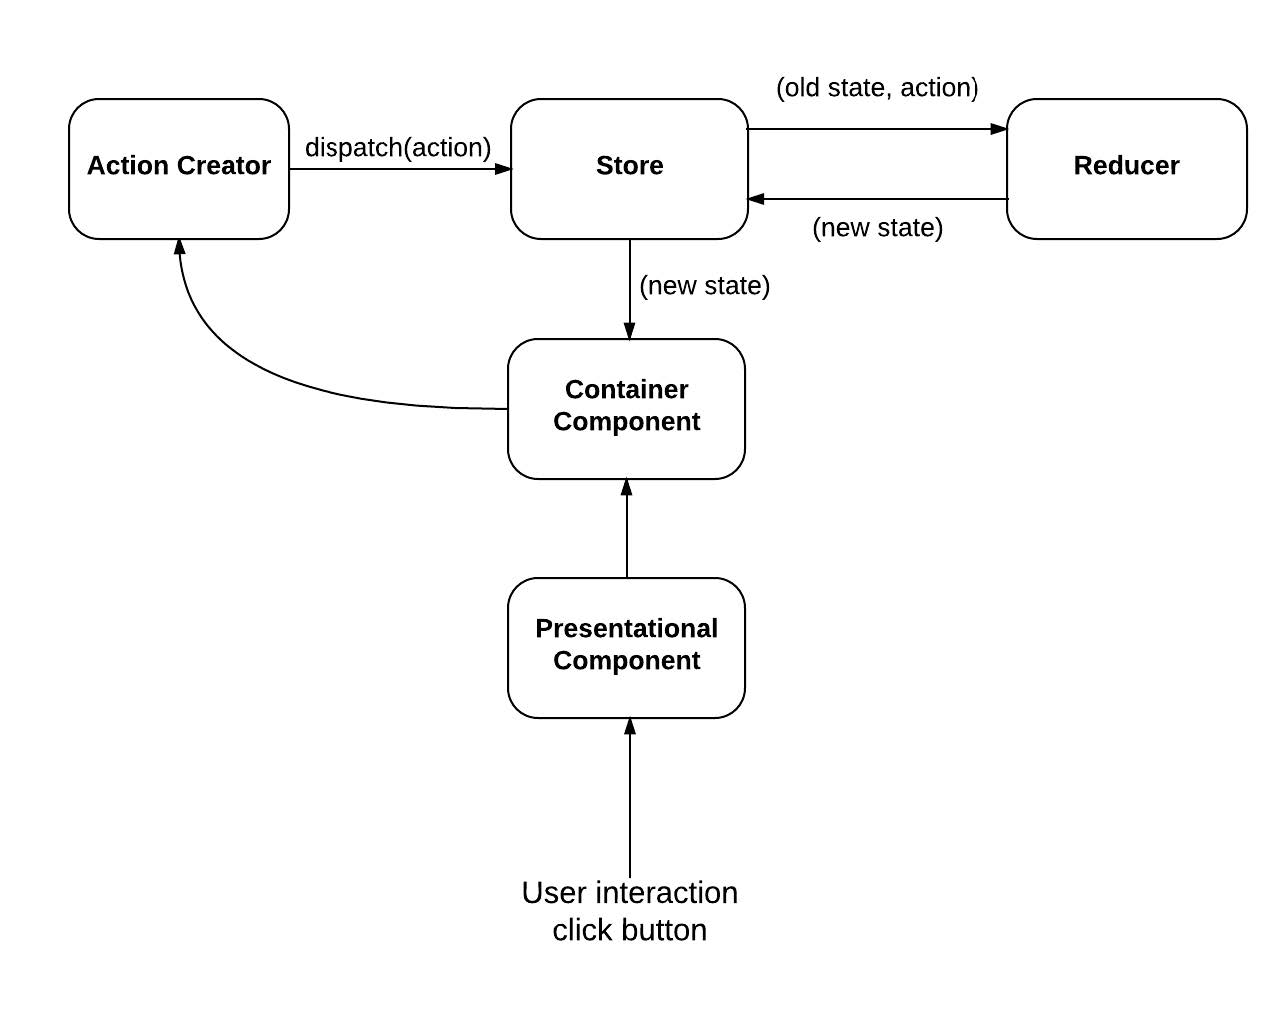
\includegraphics[scale=0.7]{figures/react-redux.png}
    \caption{Δομή \tl{React Redux} εντός της εφαρμογής.}
    \label{redux}
\end{figure}


Το κυριότερο πλεονέκτημα της \tl{React Redux} είναι ο τρόπος με τον οποίο διαχειρίζεται τα δεδομένα μιας εφαρμογής. Διαθέτει μια αμφίδρομη ροή δεδομένων μεταξύ ενός ενιαίου αποθηκευτικού χώρου και της εφαρμογής. Αυτό επιτρέπει στον προγραμματιστή τον εύκολο και γρήγορο τρόπο ανάπτυξης και αποσφαλμάτωσης της εφαρμογής.
\newline
\indent
Η δομή της εφαρμογής με τη χρήση της \tl{React Redux} φαίνεται στο σχ. \ref{redux}. Στη συνέχεια, ακολουθεί μια ανάλυση κάθε παράγοντα της βιβλιοθήκης, όπως αυτός χρησιμοποιείται εντός της εφαρμογής.

 \paragraph{\tl{\textbf{Presentational \& Container Components}}}
 \paragraph{}
 Κατά την υλοποίηση της εφαρμογής, κάθε οθόνη διακριτοποιείται σε στοιχεία αναπαράστασης δεδομένων (\tl{presentational/functional or stateless components}) και στοιχεία κατάστασης (\tl{container or ctateful components}), όπως έχει ήδη αναφερθεί στην ενότητα 4.1.4. Τα \tl{presentational components} δεν διαθέτουν λογική, το οποίο σημαίνει πως δε διαχειρίζονται καθόλου δεδομένα. Το μοναδικό συστατικό απαραίτητο στην λειτουργία τους είναι τα δεδομένα που λαμβάνουν μέσω των \tl{props} από το στοιχείο-πατέρα. Στην περίπτωση που απαιτείται η εκτέλεση μιας ενέργειας σχετική με τη διαζείριση δεδομένων από ένα \tl{presentational component}, αυτό επιτυγχάνεται με τον ίδιο τρόπο που λαμβάνονται τα δεδομένα. Με το ``\textit{πέρασμα}'' της αντίστοιχης συνάρτησης ανάκλησης (\tl{callback}) μέσω των \tl{props}, αυτή καθίσταται διαθέσιμη ανά πάσα στιγμή στο \tl{presentational component}, χωρίς την ανάγκη για πρόσθετη λογική. Κάθε \tl{presentational component} έχει την παραπάνω ιδιότητα να δέχεται δεδομένα και συναρτήσεις ώς είσοδο κατά την αρχικοποίηση.
\newline
\indent
Τα \tl{container components} είναι συνήθως στοιχεία-γονείς σε \tl{presentational components}. Αυτά αναλαμβάνουν την διαχείριση των δεδομένων και των ενεργειών που έχουν αποσταλλεί από τα \tl{presentational components}, όταν πραγματοποιείται κάποια δράση από την πλευρά του χρήστη. Επίσης, είναι υπεύθυνα για την πλοήγηση μεταξύ οθονών και πολλών άλλων σημείων λογικής εντός της εφαρμογής. 

\clearpage
 \paragraph{\tl{\textbf{Action Creators}}}
 \paragraph{}
 Για την αποστολή αιτημάτων που πυροδοτούν την εκτέλεση συγκεκριμένων ενεργειών όταν ο χρήστης αλληλεπιδρά με την εφαρμογή, η \tl{redux} χρησιμοποιεί ειδικές συναρτήσεις δημιουργίας αιτημάτων δράσεων, τους λεγόμενους \tl{action creators}. Οι \tl{action creators} χρησιμοποιούν την συνάρτηση αποστολής αιτημάτων \tl{dispatch} της \tl{redux}, που έχει εμβέλεια σε όλα τα διασυνδεδεμένα τμήματα της εφαρμογής.
 
 \paragraph{\tl{\textbf{Redux Store}}}
 \paragraph{}
 H \tl{React Redux} χρησιμοποιεί την \tl{Store} ως αποθηκευτικό χώρο για να διατηρεί την κατάσταση της εφαρμογής.  Η κατάσταση της εφαρμογής μεταβάλλεται όταν πυροδοτείται μια ενέργεια με κάποιον από τους \tl{action creators} που έχουν δημιουργηθεί για διαφορετικές ενέργειες, καθ 'όλη τη διάρκεια της εφαρμογής. Οι αλλαγές που πραγματοποιούνται αποθηκεύονται στην \tl{store}. Η κατάσταση της εφαρμογής μπορεί να οριστεί ως ένα σύνολο αντικειμένων, συλλογές από αντικείμενα, αποθηκευμένα δεδομένα από το \tl{server} και πιθανόν να υπάρχουν \tl{booleans}, \tl{integer} ή \tl{string} τιμές που ζητούνται από την εφαρμογή. Για παράδειγμα, η κατάσταση της \tl{store} της εφαρμογής μπορεί να κρατήσει την τιμή του διακριτικού ελέγχου ταυτότητας (\tl{authorization token}) ενός χρήστη, εάν ο χρήστης κατάφερε να συνδεθεί με επιτυχία στο σύστημα. Έτσι, ο χρήστης δεν χρειάζεται να επαναλαμβάνει την διαδικασία σύνδεσης στην εφαρμογή κάθε φορά που ανανεώνει την οθόνη, ή εξέρχεται προσορινά από την εφαρμογή.

 \paragraph{\tl{\textbf{Reducers}}}
 \paragraph{}
Οι \tl{Reducers} είναι αγνές συναρτήσεις (\tl{pure functions}). Έτσι ονομάζονται οι συναρτήσεις οι οποίες δεν τροποποιούν τα στοιχεία που δέχονται ως είσοδο (\tl{arguments}). Λαμβάνοντας ως είσοδο την παρούσα κατάσταση των δεδομένων της εφαρμογής, πραγματοποιούν τις απαραίτητες αλλαγές στην κατάσταση της εφαρμογής, μέσω της εκτέλεσης μιας ενέργειας που απεστάλη από κάποιον \tl{action creator}. Επιστρέφουν την νέα κατάσταση της εφαρμογής σε ένα νέο στοιχείο με τη μορφή αντικειμένου. Η νέα κατάσταση μπορεί να είναι απλά ένα αντίγραφο της προηγούμενης κατάστασης, αλλά δεν μπορεί σε καμία περίπτωση να είναι η παρούσα κατάσταση τροποποιημένη. Η παρούσα κατάσταση παραμένει πάντοτε απαράλλαχτη. Οι \tl{reducers} είναι στην ουσία μηχανές κατάστασης, οι οποίες ορίζουν τη διαδοχή μεταξύ των καταστάσεων της εφαρμογής.



\subsubsection{\tl{Redux Thunk Middleware}}
Στην περίπτωση που μια σειρά ενεργειών πρέπει να εκτελεστούν σε ένα συγκεκριμένο χρονικό σημείο που προηγείται του σταδίου των \tl{reducers}, τότε γίνεται χρήση λογισμικού ειδικού σκοπού, γνωστού ως \tl{Middleware}. Με αυτό τον τρόπο, δίνεται η δυνατότητα στον προγραμματιστή να υλοποιήσει ενδιάμεση λογική η οποία θα εκτελείται πρωτού γίνει η ενέργεια που είναι προορισμένη να πραγματοποιηθεί από κάποιον \tl{reducer} σύμφωνα με τον αντίστοιχο \tl{action creator}. 
\newline
\indent
Στην εφαρμογή γίνεται χρήση του \tl{Redux Thunk} \cite{[THUNK]}, με τη βοήθεια του οποίου ένας \tl{action creator} μπορεί να επιστρέψει μια συνάρτηση ανάκλησης \tl{callback function} στη θέση ενός αντικειμένου. Κατά τη διάρκεια εκτέλεσης του \tl{middleware}, διακόπτεται προσωρινά η ροή εκτέλεσης μιας ενέργειας για να γίνει η απαιτούμενες επεξεργασίες στην κατάσταση (βλ. Σχ. \ref{thunk}). Υπεύθυνη για το τμήμα της λογικής που εκτελείται είναι η \tl{callback function}. H \tl{callback function} εκτελείται ασύγχρονα και μόλις ολοκληρωθεί, συνεχίζεται κανονικά η ροή εκτέλεσης του προγράμματος. Έπειτα, αποστέλλεται η ενέργεια στον προοριζόμενο \tl{reducer} και η διαδικασία συνεχίζεται όπως πριν.

\begin{figure}[H]
    \centering
    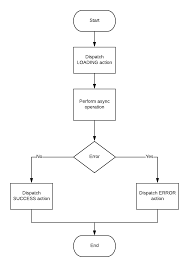
\includegraphics[scale=0.8]{figures/redux-thunk.png}
    \caption{Υλοποίηση λογικής του \tl{Redux Thunk Middleware}.}
    \label{thunk}
\end{figure}

Στην εφαρμογή, η προαναφερθείσα ροή υλοποιείται σε ενέργειες που απαιτούν τη λήψη δεδομένων από τη βάση πρωτού πυροδοτήσουν μια ενέργεια. Για παράδειγμα, όταν ο χρήστης πραγματοποιεί σύνδεση στην εφαρμογή, πυροδοτείται μια ενέργεια σύνδεσης χρήστη. Για την επιτυχή ολοκλήρωση της ενέργειας σύνδεσης θα πρέπει να γίνει λήψη των διαπιστευτηρίων του χρήστη για να διασταυρωθούν με αυτά που έδωσε ως είσοδο κατά τη διαδικασία σύνδεσης στην εφαρμογή. Έτσι, η ενέργεια σύνδεσης διακόπτεται μέχρις ότου ολοκληρωθεί το αίτημα λήψης των διαπιστευτηρίων του χρήστη από τη βάση δεδομένων. Έπειτα, η ενέργεια αποστέλλεται στον αντίστοιχο \tl{reducer} και η διαδικασία συνεχίζεται κανονικά. Στο παραπάνω παράδειγμα, η λογική που αφορά στη λήψη των διαπιστευτηρίων του χρήστη από τη βάση, αποτελεί το \tl{middleware} που εκτελείται στο ενδιάμεσο της ενέργειας σύνδεσης χρήστη στην εφαρμογή.



\subsection{Βιβλιοθήκες και Βοηθητικά Προγραμματιστικά Πακέτα}
Για την εγκατάσταση πρόσθετων βιβλιοθηκών έγινε χρήση των εργαλείων \tl{npm} και \tl{yarn}. Και τα δύο είναι βοηθητικά πακέτα διαχείρισης βιβλιοθηκών. Σκοπός τους είναι η εγκατάσταση βιβλιοθηκών και η σύνδεσή τους με τις απαραίτητες βιβλιοθήκες εξάρτησης (\tl{dependencies}) καθ' όλη την έκταση της εφαρμογής.
\newline
\indent
Στη συνέχεια θα γίνει μια αναφορά στις πιο αξιοσημείωτες βιβλιοθήκες που χρησιμοποιήθηκαν κατά την υλοποίηση της εφαρμογής.

\paragraph{\ttfamily{\tl{axios}}}
\paragraph{}
Η βιβλιοθήκη \ttfamily{\tl{axios}} χρησιμεύει για την δημιουργία και αποστολή ασύγχρονων αιτημάτων προς τον \tl{server}. Τα αιτήματα μπορούν να είναι της μορφής \ttfamily{\tl{GET, POST, PUT, DELETE}} και αναλόγως το είδος του αιτήματος μπορούν να συνοδεύονται ή όχι από δεδομένα \cite{[AXIOS]}. 


\paragraph{\ttfamily{\tl{native-base}}}
\paragraph{}
Η βιβλιοθήκη \ttfamily{\tl{native-base}} χρησιμοποιήθηκε ως επί το πλείστον για τη σχεδίαση των διεπιφανειών χρήστη της εφαρμογής. Διαδραστικά στοιχεία όπως φόρμες, πλήκτρα κλπ. έχουν σχεδιαστεί με τη βοήθεια της βιβλιοθήκης αυτής. Το χαρακτηριστικό της \ttfamily{\tl{native-base}} που την καθιστά ιδιαίτερα εξυπηρετική είναι το γεγονός ότι προσφέρει στον προγραμματιστή έτοιμα στοιχεία, τα οποία είναι ευέλικτα και πλήρως λειτουργικά. Έτσι μειώνεται σημαντικά ο απαιτούμενος χρόνος σχεδίασης και ο προγραμματιστής μπορεί να επικεντρωθεί στην υλοποίηση της λογικής της εφαρμογής \cite{[NB]}.


\paragraph{\ttfamily{\tl{react-native-router-flux}}}
\paragraph{}
Η υλοποίηση του μενού πλοήγησης εντός της εφαρμιογής έγινε με τη βοήθεια της βιβλιοθήκης \ttfamily{\tl{react-native-router-flux}}. Σύμφωνα με αυτή, κάθε οθόνη αποτελεί ένα \tl{scene} και πολλά \tl{scenes} μαζί συνιστούν ένα \tl{stack}. Κάθε \tl{scene} φέρει ιδιότητες όπως επικεφαλίδα, τίτλο, πλήκτρα πλοήγησης κλπ. Όσα \tl{scenes} βρίσκονται ομαδοποιημένα υπό ένα \tl{stack} μπορούν να διαδέχονται η μία την άλλη χάρη στην ιδιότητα μνήμης που παρέχεται στην στοίβα. Όλες οι οθόνες βρίσκονται κάτω από έναν κεντρικό δρομολογητή (\tl{router}) \cite{[RNRF]}.


\paragraph{\ttfamily{\tl{react-native-maps}}}
\paragraph{}
Η βασική βιβλιογραφία του \tl{facebook} σχετικά με τη \tl{react native} προσφέρει αυτή τη βιβλιοθήκη για την υλοποίηση διεπαφών χάρτη ως μιας καλύτερης εναλλακτικής έναντι των έτοιμων διεπαφών που υπάρχουν υλοποιημένες. Η \ttfamily{\tl{react-native-maps}} παρέχει στον προγραμματιστή μια σειρά από δυνατότητες που αφορούν στην διαμόρφωση διεπαφών χάρτη με μεγαλύτερη ευελιξία ως προς τον έλεγχο γεγονότων επάνω στο χάρτη, την μορφοποίηση της διεπιφάνειας χάρτη, την καταγραφή συντεταγμένων διαφόρων σημείων, την προγραμματισμένη μεταβολή θέσης, την χρήση διεπαφών με διαδραστικά στοιχεία και πολλά άλλα \cite{RNM}.



\subsection{Ιεράρχηση Αρχείων και Δομή Φακέλων}
Η ιεραρχία που ακολουθούν τα αρχεία δείχνει την πορεία για την κατάστρωση του σχεδίου της εφαρμογής. Υπάρχει χαρακτηριστική αντιστοιχία μεταξύ της δομής των φακέλων και της δομής της εφαρμογής. Κάθε οθόνη υλοποιείται σε ξεχωριστό φάκελο, ο οποίος περιλαμβάνει το αρχείο στο οποίο βρίσκεται ο σκελετός της συγκεκριμένης οθόνης, αλλά και τα υπόλοιπα στοιχεία που συνιστούν τα βοηθητικά \tl{components} της οθόνης. Η ονομασία των αρχείων ακολουθεί μία σύμβαση κατά την οποία τα αρχεία που περιέχουν \tl{components} ξεκινούν με κεφαλαία, ενώ οποιοδήποτε άλλο αρχείο ξεκινάει με μικρά. Αρχεία τα οποία αποτελούνται από περισσότερες από μια λέξεις ακολουθούν \tl{camelCase} γραφή (βλ. Σχ. \ref{screens}).

\begin{figure}[H]
    \centering
    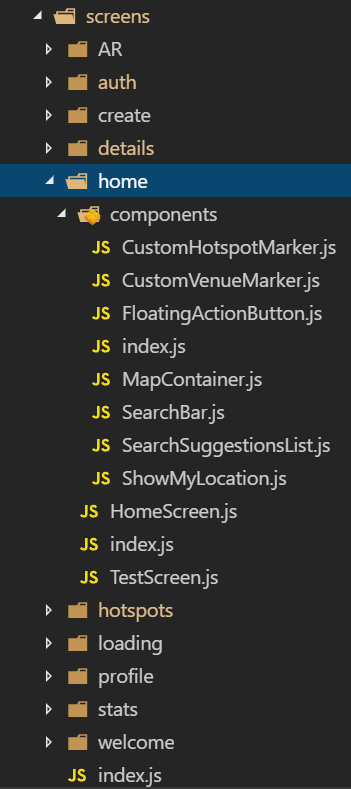
\includegraphics[scale=0.7]{figures/screens.png}
    \caption{Δομή φακέλων και αρχείων για τις οθόνες της εφαρμογής.}
    \label{screens}
\end{figure}

Η λογική που αφορά την \tl{react redux} βρίσκεται σε ξεχωριστούς φακέλους. Οι ενέργειες που πυροδοτούνται από την αλληλεπίδραση του χρήστη με τις διεπιφάνειες της εφαρμογής είναι συγκεντρωμένες στο φάκελο \tl{actions}. Κάθε \tl{action} κατατάσσεται σε διαφορετικό αρχείο, ανάλογα με το είδος του. Για παράδειγμα, \tl{actions} που αφορούν \tl{hotspots} ομαδοποιούνται σε ένα αρχείο υπό το όνομα \tl{hotspot.actions.js}. Η ίδια λογική ακολουθείται και για τα αρχεία που περιέχουν τους \tl{reducers} (βλ. Σχ. \ref{redux}).

\begin{figure}[H]
    \centering
    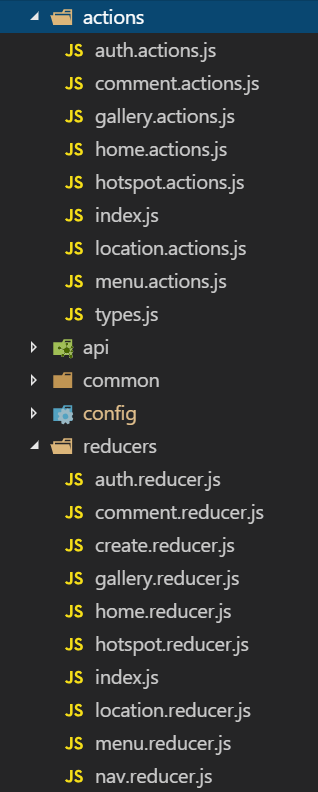
\includegraphics[scale=0.7]{figures/redux.png}
    \caption{Δομή φακέλων και αρχείων που αφορούν \tl{react redux}.}
    \label{redux}
\end{figure}

Τα αρχεία που σχετίζονται με την πλοήγηση εντός της εφαρμογής βρίσκονται σε έναν ξεχωριστό φάκελο με το όνομα \tl{routes}. Στο αρχείο με όνομα \tl{Navigator.js} βρίσκεται η υλοποίηση του κεντρικού δρομολογητή της εφαρμογής.



\section{Υλοποίηση Εξυπηρετητή Αιτημάτων και Βάσης Δεδομένων}
Σε αυτή την ενότητα θα γίνει ανάλυση των τεχνικών που εφαρμόστηκαν στην υλοποίηση του \tl{server} της εφαρμογής. Θα γίνει αναφορά στους δρομολογητές και τα αντίστοιχα \tl{routes}, καθώς και στους ελεγκτές που σχετίζονται με κάθε δρομολογητή. Θα παρουσιαστούν επίσης τα \tl{endpoints} της εφαρμογής και θα επεξηγηθούν οι λειτουργίες που αντιστοιχούν σε καθένα από αυτά.



\subsection{\tl{Server Routes}}

Ο \tl{server} χρησιμοποιεί ένα σύστημα δρομολόγησης (\tl{routes}) των αιτημάτων του \tl{client} που προορίζονται προς εξυπηρέτηση. Κάθε ομάδα υπηρεσιών που απευθύνονται σε μια συγκεκριμένη λειτουργία της εφαρμογής αντιστοιχίζεται σε ένα δρομολογητή (\tl{router}). Ο \tl{router} απαρτίζεται από επιμέρους \tl{routes}, καθεμία εκ των οποίων εξυπηρετεί μια συγκεκριμένη λειτουργία. Έτσι, στο παραπάνω παράδειγμα, το αίτημα για τη δημιουργία νέου \tl{hotspot} θα δρομολογηθεί για εξυπηρέτηση από τον \tl{router} που είναι υπεύθυνος για τις ενέργειες΄που αφορούν ένα \tl{hotspot} (\tl{\textit{HotspotRoutes}}). 

Το σύστημα των δρομολογητών έχει σχεδιαστεί με στόχο την απλότητα και την αμεσότητα στην κατανόηση από τον προγραμματιστή (βλ. Σχ. \ref{routes}). Αιτήματα που αφορούν τους χρήστες δρομολογούνται προς εξυπηρέτηση από τον \tl{router} που είναι υπεύθυνος για τις ενέργειες που αφορούν τους χρήστες. Με τον ίδιο τρόπο, Αιτήματα που σχετίζονται με σχόλια χρηστών σε ένα \tl{hotspot}, εξυπηρετούνται από εκείνο τον \tl{router} που είναι υπεύθυνος για τα σχόλια. 

\begin{figure}[h]
    \centering
    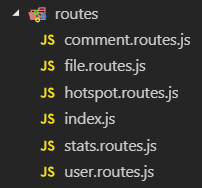
\includegraphics[scale=1]{figures/routes.png}
    \caption{Ιεράρχηση του συστήματος δρομολογητών στην εφαρμογή.}
    \label{routes}
\end{figure}

Οι δρομολογητές του συστήματος είναι οι ακόλουθοι:

\begin{itemize}
    \item \tl{\textbf{Hotspot Routes -}} περιλαμβάνει \tl{routes} που αφορούν την εξυπηρέτηση αιτημάτων σχετικά με \tl{hotspots}, όπως δημιουργία, επεξεργασία, διαγραφή, προβολή, ανάκτηση κλπ.
    \item \tl{\textbf{User Routes -}} περιλαμβάνει \tl{routes} που αφορούν την εξυπηρέτηση αιτημάτων σχετικά με χρήστες, όπως εγγραφή, σύνδεση, επεξεργασία, προβολή, ανάκτηση κλπ.
    \item \tl{\textbf{Comment Routes -}} περιλαμβάνει \tl{routes} που αφορούν την εξυπηρέτηση αιτημάτων σχετικά με σχόλια, όπως δημιουργία, προβολή, απαρίθμηση κλπ.
    \item \tl{\textbf{File Routes -}} περιλαμβάνει \tl{routes} που αφορούν την εξυπηρέτηση αιτημάτων σχετικά με συνημμένα αρχεία σε \tl{hotspots}.
    \item \tl{\textbf{Stats Routes -}} περιλαμβάνει \tl{routes} που αφορούν την εξυπηρέτηση αιτημάτων σχετικά με στατιστικά δεδομένα.
\end{itemize}

\subsection{\tl{Server Controllers}}

Αφότου τα αιτήματα δρομολογηθούν προς εξυπηρέτηση στους αντίστοιχους \tl{routers}, ακολοθεί η επεξεργασία τους και η εκτέλεσή τους μέσω κατάλληλων μεθόδων. Οι μέθοδοι που αναλαμβάνουν την εκτέλεση των αιτημάτων ονομάζονται ελεγκτές (\tl{controllers}) και αποτελούνται από ένα σύνολο ασύγχρονων εντολών και κλήσεων μεταξύ της βάσης δεδομένων και του \tl{server}.

Όπως και με το σύστημα των δρομολογητών, έτσι και οι ελεγκτές έχουν σχεδιαστεί με στόχο να αποσυμπλέκουν τις ενέργειες που σχετίζονται με κάθε αίτημα (βλ. Σχ. \ref{controllers}). Όλες οι ενέργεεις που αφορούν τα \tl{hotspots} εκτελούνται αποκλειστικά από έναν ελεγκτή. Το ίδιο συμβαίνει και με τις ενέργεεις γύρω από τους χρήστες. Το σύστημα των \tl{controllers} έχει παραπλήσια μορφή με αυτό των \tl{routers} καθώς στόχος της σχεδίασης είναι να υπάρχει ένας βαθμός αναλογίας μεταξύ των διαφόρων τμημάτων,ο οποίος μειώνει αισθητά το χρόνο κατανόησης και βελτιστοποιεί τη διαδικασία υλοποίησης:

\begin{itemize}
    \item \tl{\textbf{Hotspot Controller -}} περιλαμβάνει τις μεθόδους που αφορούν την εξυπηρέτηση αιτημάτων σχετικά με \tl{hotspots}, όπως δημιουργία, επεξεργασία, διαγραφή, προβολή, ανάκτηση κλπ.
    \item \tl{\textbf{User Controller -}} περιλαμβάνει τις μεθόδους που αφορούν την εξυπηρέτηση αιτημάτων σχετικά με χρήστες, όπως εγγραφή, σύνδεση, επεξεργασία, προβολή, ανάκτηση κλπ.
    \item \tl{\textbf{Comment Controller -}} περιλαμβάνει τις μεθόδους που αφορούν την εξυπηρέτηση αιτημάτων σχετικά με σχόλια, όπως δημιουργία, προβολή, απαρίθμηση κλπ.
    \item \tl{\textbf{File Controller -}} περιλαμβάνει τις μεθόδους που αφορούν την εξυπηρέτηση αιτημάτων σχετικά με συνημμένα αρχεία σε \tl{hotspots}.
    \item \tl{\textbf{Stats Controller -}} περιλαμβάνει τις μεθόδους που αφορούν την εξυπηρέτηση αιτημάτων σχετικά με στατιστικά δεδομένα.
    \item \tl{\textbf{Views Controller -}} περιλαμβάνει τις μεθόδους που αφορούν την εξυπηρέτηση αιτημάτων σχετικά με τα \tl{views} ενός \tl{hotspot}.
\end{itemize}

\begin{figure}[h]
    \centering
    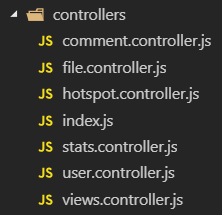
\includegraphics[scale=1]{figures/controllers-path-vscode.png}
    \caption{Ιεράρχηση του συστήματος ελεγκτών στην εφαρμογή.}
    \label{controllers}
\end{figure}

\subsection{\tl{REST API - Server Endpoints}}
Κάθε ενέργεια από την πλευρά του \tl{client} πυροδοτεί ένα αίτημα στην πλευρά του \tl{server}. Στην ενότητα αυτή αναλύεται η τεχνική με την οποία ταξινομούνται και δρομολογούνται τα αιτήματα σε συγκεκριμένα \tl{endpoints}.


\begin{itemize}
    \item \tl{hotspots}
    \newline \newline
    \textbf{\tl{\ttfamily{GET /hotspots/radius?lat=''&lng=''}}}
    \newline \newline
    \textbf{-\tl{lat}} - συντεταγμένη γεωγραφικού πλάτους (\tl{latitude}) \newline 
    \indent
    \textbf{-\tl{lng}} - συντεταγμένη γεωγραφικού μήκους (\tl{longitude})
    \newline \newline \noindent
    ανακτά όλα τα μηνύματα εντός της προκαθορισμένης ακτίνας των 5000 μέτρων από τη δεδομένη θέση που καθορίζεται από το γεωγραφικό πλάτος (\tl{lat}) και το γεωγραφικό μήκος (\tl{lng}).
    
    \newline \newline
    \textbf{\tl{\ttfamily{GET /hotspots/:hospotId}}}
    \newline \newline \noindent
    ανακτά τις πληροφορίες που αφορούν το μηνύμα με το συγκεκριμένο αναγνωριστικό \tl{hotspotId}.
    
    \newline \newline
    \textbf{\tl{\ttfamily{GET /users/:userId/hotspots}}}
    \newline \newline \noindent
    ανακτά όλα τα μηνύματα του χρήστη με το συγκεκριμένο αναγνωριστικό \tl{userId}.
    
    \newline \newline
    \textbf{\tl{\ttfamily{POST /hotspots/new}}}
    \newline \newline \noindent
    δημιουργεί μια νέα είσοδο για την αποθήκευση ενός καινούριου \tl{hotspot} στη βάση.
    
    \newline \newline
    \textbf{\tl{\ttfamily{PUT /hotspots/:hotspotId/edit}}}
    \newline \newline \noindent
    επεξεργάζεται το \tl{hotspot} με το προκαθορισμένο αναγνωριστικό \tl{hotspotId}, με τα δοθέντα στοιχεία.
    
    \newline \newline
    \textbf{\tl{\ttfamily{DELETE /hotspots/:hotspotId/delete}}}
    \newline \newline \noindent
    διαγράφει το \tl{hotspot} με το προκαθορισμένο αναγνωριστικό \tl{hotspotId} από τη βάση δεδομένων.
    
    \item \tl{users}
    
    \newline \newline
    \textbf{\tl{\ttfamily{GET /users/:userId}}}
    \newline \newline \noindent
    ανακτά τα στοιχεία του χρήστη που προσδιορίζεται από το αναγνωριστικό \tl{userId}.
    
    \newline \newline
    \textbf{\tl{\ttfamily{POST /register}}}
    \newline \newline \noindent
    πραγματοποιεί εγγραφή ενός νέου χρήστη στο σύστημα, τα αποθηκεύει τα στοιχεία στη βάση και εκδίδει σύμβολο ταυτοποίησης (\tl{access token}).
    
    \newpage
    \newline \newline
    \textbf{\tl{\ttfamily{POST /login}}}
    \newline \newline \noindent
    πραγματοποιεί σύνδεση ενός χρήστη στην εφαρμογή και εκδίδει σύμβολο ταυτοποίησης (\tl{access token}).
    
    \newline \newline
    \textbf{\tl{\ttfamily{POST /verify}}}
    \newline \newline \noindent
    πραγματοποιεί έλεγχο της ταυτότητας του χρήστη διασταυρώνοντας το σύμβολο ταυτοποίησης του χρήστη με αυτό που είναι αποθηκευμένο στη βάση.
    
    \newline \newline
    \textbf{\tl{\ttfamily{PUT /users/:userId/edit}}}
    \newline \newline \noindent
    επεξεργάζεται τα στοιχεία του χρήστη που καθορίζεται από το αναγνωριστικό \tl{userId} και αποθηκεύει τον ανανεωμένο χρήστη στη βάση.
    
    \item \tl{comments}
    
    \newline \newline
    \textbf{\tl{\ttfamily{GET /:userId/hotspots/:hotspotId/comments}}}
    \newline \newline \noindent
    ανακτά τα σχόλια ενός \tl{hotspot} με τη βοήθεια των διακριτικών \tl{hotspotId} και \tl{userId}.
    
    \newline \newline
    \textbf{\tl{\ttfamily{POST /:userId/hotspots/:hotspotId/comments/new}}}
    \newline \newline \noindent
    δημιουργεί μια είσοδο στη βάση για την αποθήκευση ενός καινούριου σχολίου. Χρειάζεται το αναγνωριστικό του \tl{hotspot} στο οποίο έγινε το σχόλιο, καθώς επίσης και του διακριτικού του χρήστη που έκανε το σχόλιο.
    
    \item \tl{files}
    
    \newline \newline
    \textbf{\tl{\ttfamily{GET /users/:userId/gallery}}}
    \newline \newline \noindent
    ανακτά όλα τα αρχεία ενός χρήστη με το συγκεκριμένο αναγνωριστικό \tl{userId}.
    
    \newline \newline
    \textbf{\tl{\ttfamily{POST /users/:userId/gallery/upload}}}
    \newline \newline \noindent
    δημιουργεί μια νέα είσοδο στη βάση για την αποθήκευση ενός αρχείου που αφορά το χρήστη με το συγκεκριμένο αναγνωριστικό \tl{userId}.
    
    \newline \newline
    \textbf{\tl{\ttfamily{DELETE /gallery/:fileId/delete}}}
    \newline \newline \noindent
    διαγράφει το αρχείο με το προκαθορισμένο αναγνωριστικό \tl{fileId} από τη βάση δεδομένων όταν διαγραφεί ένα \tl{hotspot}.
    
    \item \tl{stats}
    
    \newline \newline
    \textbf{\tl{\ttfamily{GET /stats/users}}}
    \newline \newline \noindent
    ανακτά το συνολικό αριθμό των χρηστών που χρησιμοποιούν την εφαρμογή.
    
    \newline \newline
    \textbf{\tl{\ttfamily{GET /stats/comments}}}
    \newline \newline \noindent
    ανακτά το συνολικό αριθμό των σχολίων που έχουν δημιουργηθεί εντός της εφαρμογής.
    
    \newline \newline
    \textbf{\tl{\ttfamily{GET /stats/hotspots}}}
    \newline \newline \noindent
    ανακτά το συνολικό αριθμό των \tl{hotspots} που έχουν δημιουργηθεί εντός της εφαρμογής.
    
    \newline \newline
    \textbf{\tl{\ttfamily{GET /stats/views}}}
    \newline \newline \noindent
    ανακτά το συνολικό αριθμό των \tl{views} που έχουν δημιουργηθεί εντός της εφαρμογής.
    
    \newline \newline
    \textbf{\tl{\ttfamily{GET /stats/:userId/hotspots}}}
    \newline \newline \noindent
    ανακτά το συνολικό αριθμό των \tl{hotspots} που έχουν δημιουργηθεί από τον χρήστη με το συγκεκριμένο αναγνωριστικό \tl{userId}.
    
    \newline \newline
    \textbf{\tl{\ttfamily{GET /stats/:userId/comments}}}
    \newline \newline \noindent
    ανακτά το συνολικό αριθμό των σχολίων που έχουν δημιουργηθεί από τον χρήστη με το συγκεκριμένο αναγνωριστικό \tl{userId}.
    
    \newline \newline
    \textbf{\tl{\ttfamily{GET /stats/:userId/ratio}}}
    \newline \newline \noindent
    ανακτά το ποσοστό αγοριών/κοριτσιών που έχουν προβάλλει τα \tl{hotspots} του χρήστη με το συγκεκριμένο αναγνωριστικό \tl{userId}.
    
   
\end{itemize}

\subsubsection{Βιβλιοθήκες και Βοηθητικά Προγραμματιστικά Πακέτα}
Για την εγκατάσταση πρόσθετων βιβλιοθηκών έγινε και εδώ χρήση των εργαλείων \tl{npm} και \tl{yarn}. Στη συνέχεια θα γίνει μια αναφορά στις πιο αξιοσημείωτες βιβλιοθήκες που χρησιμοποιήθηκαν κατά την υλοποίηση του εξυπηρετητή και της βάσης δεδομένων.

\paragraph{\ttfamily{\tl{passport}}}
\paragraph{}
Η βιβλιοθήκη \ttfamily{\tl{passport}} αποτελεί ένα είδος \tl{middleware} για την ταυτοποίηση χρηστών. Χρησιμοποιώντας τεχνικές ταυτοποίησης που ονομάζονται \tl{strategies}, καθορίζει τον τρόπο με τον οποίο γίνεται η ταυτοποίηση χρηστών στα διάφορα σενάρια που περιλαμβάνει η εφαρμογή \cite{[PASSPORT]}. 


\paragraph{\ttfamily{\tl{babel}}}
\paragraph{}
Η βιβλιοθήκη \ttfamily{\tl{babel}} χρησιμοποιήθηκε ως ο βασικός μεταγλωττιστής του κώδικα από \tl{ES6} σε \tl{ES5}. Η \ttfamily{\tl{babel}} υποστηρίζει την πιο πρόσφατη έκδοση \tl{JavaScript} χρησιμοποιώντας συντακτικούς μετατροπείς (\tl{syntax transformers}) \cite{[BABEL]}.


\paragraph{\ttfamily{\tl{mongoose}}}
\paragraph{}
Η βιβλιοθήκη \ttfamily{\tl{mongoose}} χρησιμοποιήθηκε για την προσθήκη κάποιων βασικών ιδιοτήτων στην βάση δεδομένων. Τέτοιες είναι η μοντελοποίηση της βάσης σε \tl{models} με συγκεκριμένη δομή. Εξίσου σημαντική είναι η δυνατότητα σελιδοποίησης των \tl{collections} εντός της βάσης και η επιστροφή σελιδοποιημένων αποτελεσμάτων σε κάθε αναζήτηση \cite{[MONGOOSE]}. 


\paragraph{\ttfamily{\tl{bcryptjs}}}
\paragraph{}
Η βιβλιοθήκη \ttfamily{\tl{bcryptjs}} χρησιμοποιείται για την κρυπτογράφηση ευαίσθητων πληροφοριών που αποθηκεύονται στη βάση δεδομένων. Συνήθως χρησιμεύει για την κρυπτογράφηση κωδικών πρόσβασης και την αποφυγή κατάχρησής τους από κακόβουλο λογισμικό \cite{[BCRYPT]}.





\section{\tl{Expo SDK \& Expo Client}}
Η ανάπτυξη \tl{iOS} εφαρμογών γίνεται μόνο στις αντίστοιχες \tl{iOS} πλατφόρμες. Για την υλοποίηση εφαρμογών σε άλλες πλατφόρμες (πχ. \tl{Windows}) είναι απαραίτητη η χρήση ενός ενδιάμεσου λογισμικού για την φιλοξενία της εφαρμογής. Το \tl{Expo} είναι διαμορφωμένο ώστε να διευκολύνει τον προγραμματιστή με τον ταυτοχρονισμό της ανάπτυξης εφαρμογών και ελέγχου λειτουργίας.
\newline
\indent
Το \tl{Expo SDK} παρέχει στον προγραμματιστή όλες τις μητρικές διεπαφές που διατίθενται στις μητρικές γλώσσες προγραμματισμού. Τα βασικά \tl{APIs} όπως η κάμερα, οι ειδοποιήσεις, η τοποθεσία, η συλλογή φωτογραφιών κλπ. μπορούν να χρησιμοποιηθούν άμεσα, χωρίς πρόσθετη λογική, όπως θα γινόταν στον προγραμματισμό σε \tl{Swift}. Στόχος του λογισμικού είναι να εξομαλύνει όσο το δυνατό περισσότερο την εμπειρία προγραμματισμού, αλλά και την εμπειρία χρήσης των διεπιφανειών, μειώνοντας τις διαφορές στο ελάχιστο. Η πλατφόρμα προσπαθεί να καλύπτει όλα τα δυνατά σενάρια χρήσης που εμφανίζονται στις σύγχρονες εφαρμογές, καθιστώντας των κώδικα πλήρως δυναμικό.
\newline
\indent
Με την εγκατάσταση του \tl{Expo Client} σε μια συσκευή \tl{iOS} ο προγραμματιστής μπορεί να πραγματοποιεί έλεγχο σε πραγματικό χρόνο. Ο \tl{Expo Client} φιλοξενεί την υπό ανάπτυξη εφαρμογή σε ένα περιβάλλον ειδικά διαμορφωμένο για αυτό τον σκοπό. Κατά τον έλεγχο της εφαρμογής, εμφανίζονται ειδικά μηνύματα σφάλματος στον προγραμματιστή που βοηθάνε στη διαδιακσία αποσφαλμάτωσης της εφαρμογής σε πραγματικό χρόνο. Έτσι, μειώνεται σε μεγάλο βαθμό η δυσκολία εύρεσης σφαλμάτων στον κώδικα, καθώς και ο χρόνος αποσφαλμάτωσης της εφαρμογής.


\section{\tl{Visual Studio Code}}

Η πλατφόρμα προγραμματισμού που προτιμήθηκε στην ανάπτυξη της εφαρμογής ήταν το \tl{VSCode} της \tl{\textit{Microsoft}}. Η επιλογή βασίστηκε στις αμέτρητες δυνατότητες που προσφέρει η πλατφορμα αυτή. Σημαντικοί παράγοντες αποτέλεσαν επίσης η ευελιξία στον τρόπο προγραμματισμού, η αυξημένη ελαστικότητα ως προς τη διαμόρφωση του περιβάλλοντος προγραμματισμού εντός της πλατφόρμας, καθώς επίσης και η μεγάλη υποστήριξη που λαμβάνει η πλατφόρμα από την παγκόσμια προγραμματιστική κοινότητα.
